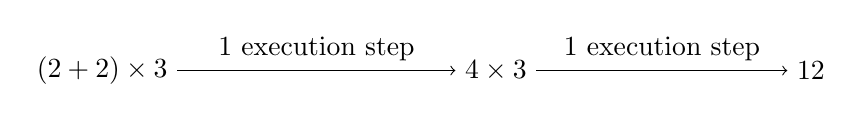
\begin{tikzpicture}[->]

\node (v1) at (-7,0) {$ (2+2) \times 3$};
\node (v2) at (-2,0) {$ 4 \times 3$};
\node (v3) at (2,0) {$ 12 $};
\draw  (v1) -- (v2) node[midway,above] {1 execution step};
\draw  (v2) -- (v3) node[midway,above] {1 execution step};
%\draw (-8.5,-1.5) -- (2.5,-1.5) node[above] {$t$};
\end{tikzpicture}